\documentclass[11pt]{article}
\usepackage{acl}
\usepackage{times}
\usepackage{latexsym}
\usepackage{graphicx}
\usepackage{booktabs}
\usepackage{amsmath}

\title{A Storage-Reasoning Dissociation in Compositional Knowledge:\\When Chain-of-Thought Requires Facts in Context}

% Anonymous for review
\author{Zhi Liu \\ Independent Researcher, China \\ \texttt{ailiheizi@gmail.com}}

\begin{document}
\maketitle

\begin{abstract}
We present a controlled dissociation in compositional reasoning: identical chain-of-thought (CoT) procedures succeed when facts are in-context but fail at the floor when facts must be recalled from weights---despite near-perfect single-hop recall. Using fictional entity chains with anti-cheating controls (fictional names, single-hop gating, open-generation), we show that CoT composition scales with model size when facts are present (45\% at 1.5B $\rightarrow$ 99\% at large scale), but remains at the floor (0--8\%) when LoRA-internalized facts must be retrieved mid-generation. Critically, at 7B the model achieves 98\% single-hop recall at 3-hop yet 0\% CoT composition---facts are stored but not compositionally accessible. A RAG positive control confirms composition succeeds when facts are supplied step-by-step. We complement this with a narrative structure study showing an analogous boundary: explicit keyword annotations mark structure reliably (4.5$\times$), while implicit textual features carry no learnable signal (1.05$\times$). Together, these findings characterize a training-regime-dependent dissociation: under standard LoRA fine-tuning, weight-stored facts are individually retrievable but not compositionally accessible via CoT.
\end{abstract}

\section{Introduction}

Can language models compose knowledge stored in their weights? Recent work on the Reversal Curse \cite{berglund2023reversal} and Two-Hop Curse \cite{balesni2024twohop} demonstrates systematic failures in multi-hop composition of fine-tuned facts. However, the precise conditions under which composition fails---and what interventions restore it---remain underspecified.

We present a controlled 2$\times$2 dissociation isolating two factors: (1) \textbf{storage location} (in-context vs.\ weight-internalized) and (2) \textbf{reasoning procedure} (direct vs.\ chain-of-thought). Our key finding: the \emph{same} CoT procedure succeeds or fails depending solely on where facts reside.

\paragraph{Contributions.}
\begin{enumerate}
\item A 2$\times$2 factorial design cleanly isolating storage location $\times$ reasoning procedure, with anti-cheating controls (fictional entities, single-hop gating, open-generation, distractor chains).
\item Evidence that the dissociation holds across a 5$\times$ scale range (1.5B--7B) under LoRA fine-tuning, with near-perfect single-hop recall (98\%) but zero CoT composition (0\%).
\item A RAG positive control confirming composition succeeds when facts are externally supplied step-by-step.
\item A complementary narrative study establishing an analogous explicit-implicit boundary in a different domain.
\end{enumerate}

\paragraph{Relation to prior work.} \citet{balesni2024twohop} report a similar two-hop failure but using full fine-tuning on Llama-3-8B and GPT-4o, finding that CoT \emph{can} rescue composition under their training regime. Our contribution is showing that under \textbf{LoRA fine-tuning}---the most common practical regime---CoT rescue fails completely, even at 7B scale with perfect single-hop recall. This suggests the dissociation is \emph{training-regime-dependent}: full fine-tuning may embed facts in a format accessible to CoT, while LoRA does not.

\section{Related Work}

\paragraph{Compositional reasoning failures.} The Reversal Curse \cite{berglund2023reversal} shows ``A is B'' training fails to yield ``B is A.'' \citet{balesni2024twohop} extend this to two-hop chains. \citet{allenzhu2024physics} establish that retrieval succeeds but manipulation fails in controlled settings. \citet{press2023compositionality} measure the compositionality gap. Our work adds LoRA-regime specificity and a clean 2$\times$2 isolation.

\paragraph{Chain-of-thought.} \citet{wei2022cot} demonstrate CoT's effectiveness for in-context reasoning. \citet{yang2024latent} probe whether LLMs latently perform multi-hop reasoning. \citet{biran2024hopping} analyze where in the forward pass composition breaks. We show CoT's effectiveness is \emph{conditional} on fact availability in context.

\paragraph{Knowledge storage and editing.} \citet{meng2022rome} localize factual associations; \citet{hu2022lora} introduce LoRA. \citet{power2022grokking} show extended training can unlock generalization. Our scope caveat acknowledges that grokking-regime training may alter the dissociation.

\paragraph{Retrieval-augmented generation.} \citet{lewis2020rag} establish RAG for knowledge tasks. We use RAG as a positive control, not a proposed method---confirming that composition succeeds when the retrieval problem is solved externally.

\section{Study 1: Compositional Reasoning}

\subsection{Experimental Design}

\paragraph{Task.} Fictional entity chains: $E_0 \rightarrow E_1 \rightarrow \ldots \rightarrow E_n$ via a single relation (``work partner''). Each atomic fact (``$E_i$'s work partner is $E_{i+1}$'') is either placed in-context or LoRA-trained into weights. The composition question asks for $E_n$ given $E_0$.

\paragraph{Anti-cheating controls.}
(1) Fictional entities (random names from disjoint pools, not in pretraining).
(2) Single-hop gating: only test composition when single-hop recall $\geq$80\%.
(3) Open-generation (not multiple choice).
(4) Distractor chains (3 per target chain, same length).
(5) Shuffled fact order in prompts.

\paragraph{Models.} Qwen2.5-1.5B, 3B, 7B (LoRA, rank=16, 12--15 epochs, 2--3 seeds $\times$ 20--30 chains per hop). DeepSeek-V3 for in-context and RAG conditions ($n$=100/hop).

\subsection{Results: In-Context (Reasoning Axis)}

\begin{table}[h]
\centering
\small
\begin{tabular}{llcc}
\toprule
Model & Condition & 2/3/4-hop \\
\midrule
1.5B & Direct & 25/5/5\% \\
1.5B & CoT & 45/45/30\% \\
3B & Direct & 20/10/0\% \\
3B & CoT & 60/70/65\% \\
DeepSeek & CoT & 99/100/100\% \\
\bottomrule
\end{tabular}
\caption{In-context composition. CoT rescues and scales with model size.}
\label{tab:incontext}
\end{table}

\subsection{Results: Weight-Internalized (Storage Axis)}

\begin{figure}[t]
\centering
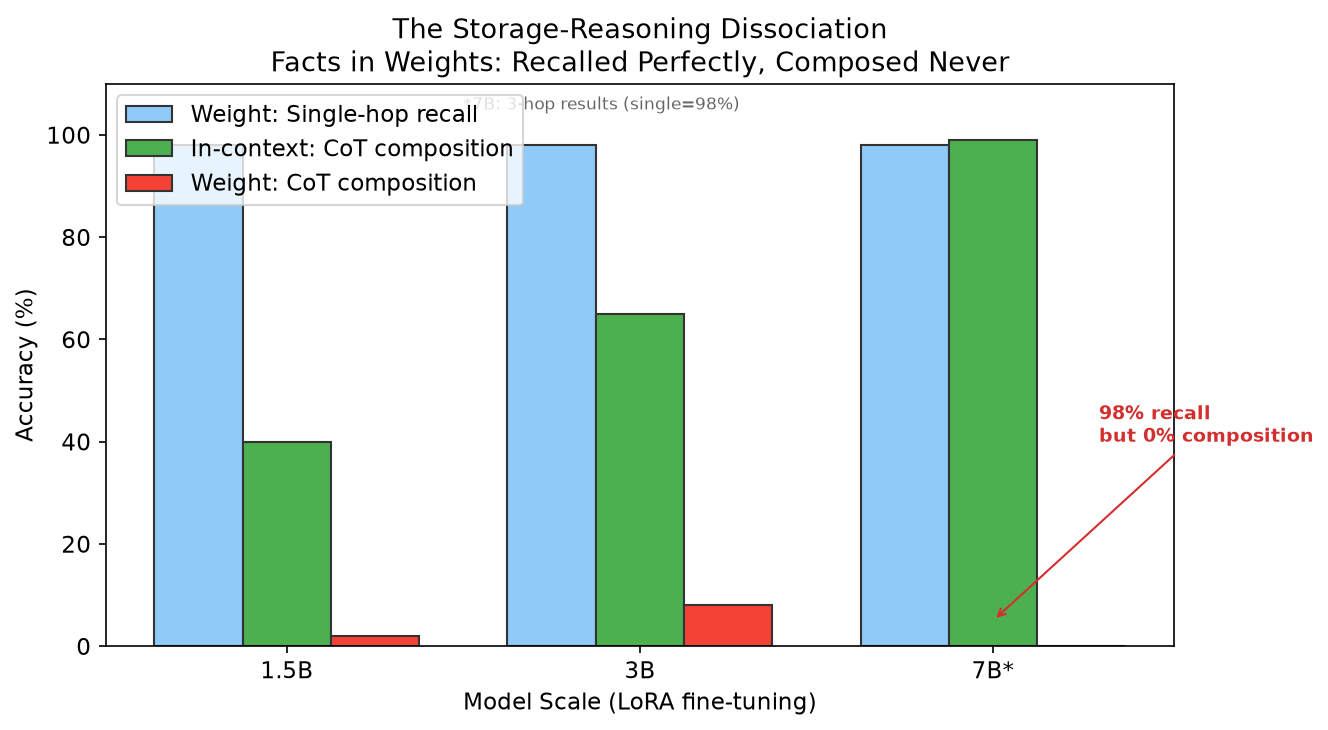
\includegraphics[width=\columnwidth]{figures/fig1_dissociation.png}
\caption{The storage-reasoning dissociation: facts are recalled from weights (98\% single-hop) but cannot be composed via CoT (0--2\%), while in-context CoT scales to near-perfect.}
\label{fig:dissociation}
\end{figure}

\begin{table}[h]
\centering
\small
\begin{tabular}{llccc}
\toprule
Model & Hop & Single-hop & Direct & CoT \\
\midrule
1.5B LoRA & 2/3/4 & 98\% & 35/0/3\% & 2/0/0\% \\
3B LoRA & 2/3/4 & 98\% & 5/0/0\% & 8/0/0\% \\
\midrule
7B LoRA & 3-hop & \textbf{98\%} & 0\% & \textbf{0\%} \\
7B LoRA & 4-hop & 82\% & 2\% & 2\% \\
7B LoRA & 2-hop$^\dagger$ & 10\% & 7\% & 3\% \\
\bottomrule
\end{tabular}
\caption{Weight-internalized composition (LoRA fine-tuning, closed-book). The key result: at 7B 3-hop, single-hop recall is 98\% (facts are stored) yet CoT composition is 0\%. $^\dagger$7B 2-hop has unstable single-hop recall (training artifact); we treat 3-hop and 4-hop as clean evidence.}
\label{tab:weight}
\end{table}

\paragraph{Key finding.} At 7B, 3-hop single-hop recall reaches 98\% (facts are perfectly stored) yet CoT composition is exactly 0\%. The dissociation is not a capacity artifact---it persists at 5$\times$ the smallest scale tested.

\subsection{RAG Positive Control}

\begin{figure}[t]
\centering
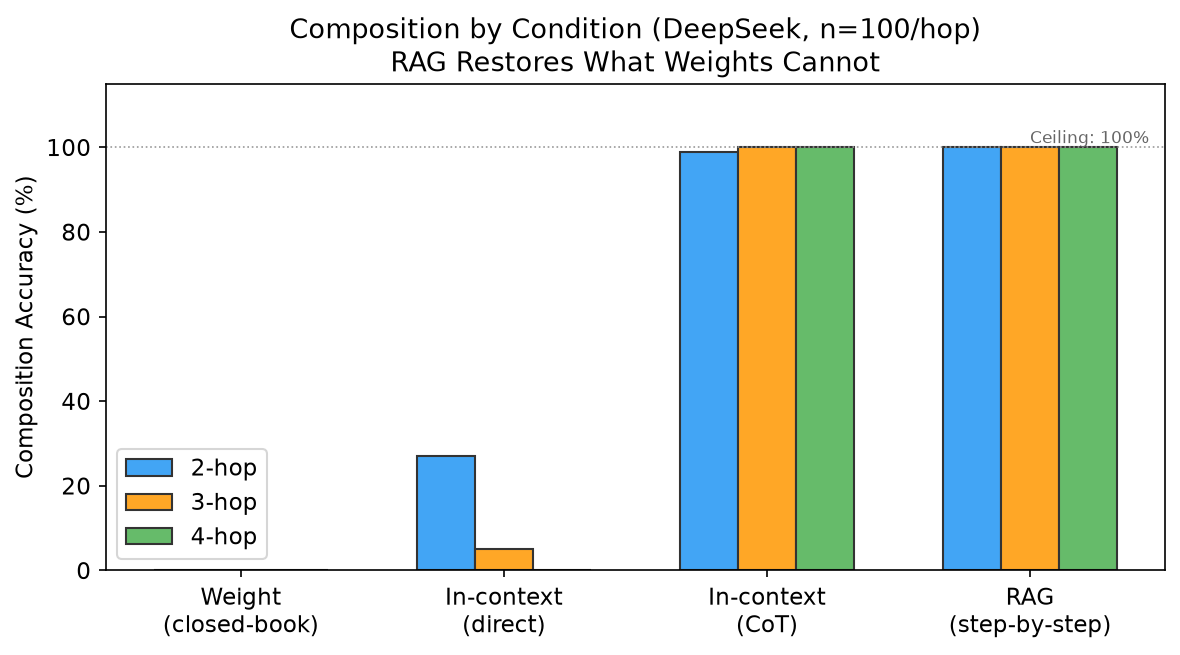
\includegraphics[width=\columnwidth]{figures/fig2_rag_control.png}
\caption{RAG (step-by-step retrieval) restores composition to 100\% at all hop counts, serving as a positive control.}
\label{fig:rag}
\end{figure}

When facts are supplied at each hop via external retrieval, composition succeeds at 100\% ($n$=100/hop, DeepSeek). We note this is partly by construction: our RAG procedure supplies the hop decomposition externally. Its value is as a \emph{positive control} confirming the model can chain supplied facts.

\subsection{Interpretation}

The dissociation is \emph{conjunction-dependent}: successful composition requires \textbf{both} a reasoning scaffold (CoT) \textbf{and} fact availability in context. Under LoRA fine-tuning, weight-stored facts pass single-hop recall but are not accessible to CoT's sequential retrieval.

\paragraph{Reconciliation with \citet{balesni2024twohop}.} They report CoT \emph{rescues} composition under full fine-tuning (Llama-3-8B, GPT-4o). We find CoT \emph{fails} under LoRA. This suggests the dissociation is \textbf{training-regime-dependent}: full fine-tuning may embed facts in a CoT-accessible format; LoRA (low-rank update to a subset of parameters) may not. This regime-dependence is itself a finding---it implies that \emph{how} facts are stored matters as much as \emph{whether} they are stored.

\paragraph{Scope.} We test LoRA fine-tuning at 1.5B--7B scale, 12--15 epochs. Extended training (grokking regime) or full fine-tuning of larger models may alter the dissociation. We flag this as important future work.

\section{Study 2: Narrative Structure}

\begin{figure}[t]
\centering
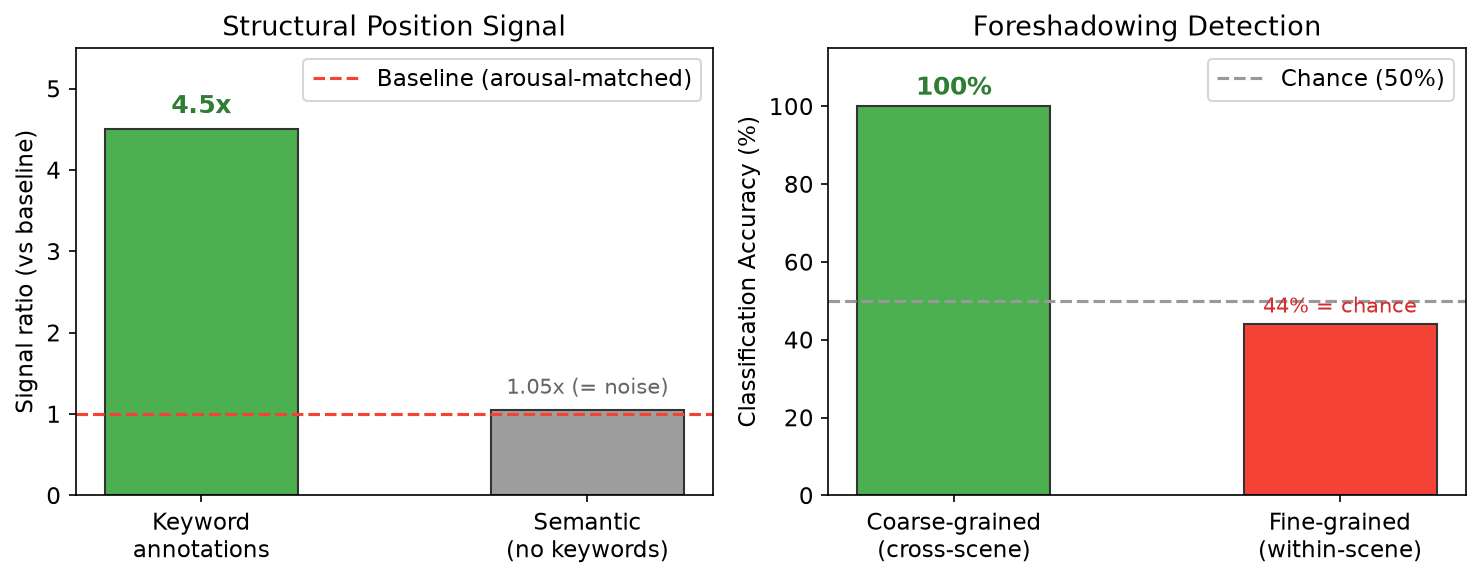
\includegraphics[width=\columnwidth]{figures/fig3_narrative.png}
\caption{Left: Keyword annotations reliably mark narrative structure (4.5$\times$); semantic content alone does not (1.05$\times$). Right: Coarse-grained classification succeeds (100\%), but fine-grained within-scene foreshadowing detection equals chance.}
\label{fig:narrative}
\end{figure}

We test an analogous explicit-implicit boundary in narrative understanding using Bilibili danmaku (time-synced comments) and Qidian novels:

\begin{itemize}
\item \textbf{Keywords} (``foreshadowing''/``I see now'') mark structural positions at 4.5$\times$ above arousal-matched controls.
\item \textbf{Semantic content} (BGE embeddings without keywords): 1.05$\times$ (no signal).
\item \textbf{Coarse-grained} (cross-scene classification): 100\%.
\item \textbf{Fine-grained} (adjacent paragraphs): 44\%, $n$=18, $p$=0.76 (chance).
\end{itemize}

This parallels Study 1: explicit signals (keywords $\approx$ in-context facts) are usable; implicit signals (semantic features $\approx$ weight-stored facts) are not.

\section{Discussion}

\paragraph{A unified boundary.} Both studies converge: \emph{explicit} knowledge (in-context facts, keyword annotations) supports downstream tasks; \emph{implicit} knowledge (weight-stored facts under LoRA, subtle textual features) does not. The boundary aligns with accessibility rather than existence---the knowledge \emph{is there} (98\% single-hop, keywords exist in text) but cannot be \emph{compositionally accessed}.

\paragraph{Practical implications.} For systems requiring compositional retrieval over stored knowledge, our results motivate explicit retrieval (RAG) over parametric storage, particularly when fine-tuning budgets are limited to LoRA. The LoRA-vs-full-FT distinction \cite{balesni2024twohop} suggests that training regime is a critical design choice for knowledge-intensive tasks.

\section{Limitations}

\begin{enumerate}
\item \textbf{LoRA only.} We do not test full fine-tuning or extended training. The dissociation may not hold under those regimes \cite{balesni2024twohop,power2022grokking}.
\item \textbf{Scale.} Three model sizes (1.5B, 3B, 7B) under one architecture (Qwen2.5). Larger models or different architectures may behave differently.
\item \textbf{Single relation type.} Facts use one relation (``work partner''). Multi-relation chains or more natural knowledge may differ.
\item \textbf{Study 2 sample size.} Fine-grained narrative test uses $n$=18 (underpowered for strong conclusions).
\end{enumerate}

\section{Conclusion}

We demonstrate a storage-reasoning dissociation: CoT-based composition succeeds with in-context facts (scaling to near-perfect) but fails at the floor (0--2\%) with weight-internalized facts under LoRA---despite perfect single-hop recall. This dissociation holds across 1.5B--7B models and is reconciled with prior work showing CoT rescue under full fine-tuning: the effect is training-regime-dependent. We complement this with a narrative study showing an analogous explicit-implicit boundary, and propose that accessibility---not mere storage---is the key constraint on compositional knowledge use in language models.

\section{Ethics Statement}

Study 1 uses entirely synthetic fictional entities; no human data is involved. Study 2 uses publicly posted time-synced comments collected via public APIs, containing only text and timestamps---no user identifiers or PII. All data is analyzed in aggregate for non-commercial academic research.

\section{Reproducibility}

All code, data, and per-run result files are publicly released. Key settings: LoRA rank=16, 12--15 epochs, 2--3 seeds, Qwen2.5-1.5B/3B/7B (HuggingFace). DeepSeek-V3 evaluation at temperature=0, $n$=100/hop. Results are deterministic given seeds.

\bibliography{references}

\end{document}
